\chapter{无人机目标识别与跟踪方法研究}
\label{chap:main}
本章将进入论文排版的正文, 按元素分主要包括:
{\kai 字体段落,图片表格,公式定理,参考文献}这几部分。
这个样例文件将包括模板中使用到的所有格式、模板中自定义命令到或者特有的东西,
都将被一一介绍,希望大家在排版自己的学位论文前能细致的看一遍,记住样例的格式和
方法,方便上手。
\cite{ELIDRISSI94}

\section{引言}
针对目标监测问题,很多学者提出了不同的解决方法,但目标实时监测问题中的所涉及的目标尺度变化、被遮挡和实时性等问题仍然没有得到有效解决。


\section{基于角点检测的目标跟踪方法研究}



\section{基于主动态轮廓线的轮廓线的目标跟踪方法研究}



\section{基于Tracking-Learning-Detection的目标跟踪方法研究}
\subsection{Tracking-Learning-Detection基本框架}
TLD(Tracking-Learning-Detection)是一种针对单一目标的长时间跟踪算法(long-term tracking)。对于一段长时间的视频,我们希望对其中某个目标进行跟踪(一个人,一辆车,或者仅仅是一块运动的区域),首先在某一帧画面规定一个矩形框,框住的区域就是我们关注的目标,那么该算法做的事就是在接下来的视频中不断跟踪这个目标,无论该物体是否暂时离开画面,或者被遮挡,或者发生形变,都不会影响继续的跟踪。该框架包含这样三个部分:
\begin{itemize}
	\item 1. 跟踪器(Tracker),通过连续帧图像来预估所追踪对象的运动,这里假设帧与帧之间目标的相对运动有限,并且追踪目标保持在图像中始终可见。追踪器可能会出现追踪失败的情形,并且在目标跳出相机视野后无法恢复追踪。
	\item 2. 检测器(Detector),将各帧图像视为独立,并对每一帧图像都进行全扫面,以找出图像中所有与目标外貌相似的候选样本。该探测器会产生两类错误:错误的正样本(False Positives)和错误的负样本(False Negatives)。
	\item 3. 学习(Learning),学习过程实时观测追踪器和探测器的执行,并预估探测器的错误,生成训练样例以使能在未来避免类似的错误。学习组件假设追踪器和探测器都有可能出现失败执行,但学习组件的引入可以使得探测器生成更多的追踪目标外观,以区别背景。
\end{itemize}
\subsection{跟踪器的设计}
\subsubsection{前向后向传播算法}

\subsection{检测器的设计}
将各帧图像视为独立,并对每一帧图像都进行全扫面,以找出图像中所有与目标外貌相似的候选样本,候选样本的生成来自学习模块。该探测器会产生两类错误:错误的正样本(false positives)和错误的负样本(false negatives)。

\subsubsection{检测区域的生成}
检首先介绍一下基本的检测区域的生成和选择,即扫描窗网格。我们通过以下参数生成所有可能比例(scales)和转移(shifts)的初始边界框:比例step=1.2,水平step=10(百分比宽度),竖直step=10(百分比高度),最小边界框大小为20像素。针对一个图像(240*320)们可以生成约50K个边界框,准确数字需要基于初始边界框的宽高比。

\subsubsection{正样本区域的放射变换}
对每个正样本区域,进行$±1\%$范围的偏移,$±1\%$范围的尺度变化,$±10\%$范围的平面内旋转,并且在每个像素上增加方差为5的高斯噪声(确切的大小是在指定的范围内随机选择的),那么每个box都进行20次这种几何变换,那么10个box将产生200个仿射变换的bounding box,作为正样本。

\subsubsection{级联分类器的设计}
是由三个串行级联的三个部分组成,即级联分类器(Cascaded Classifier)。由于需要评估的边界框数量较多,每个单独的片段分类过程需要做到十分高效。如下图所示,我们将分类设计为三个阶段:图像变化(patch variance)、总体分类(ensemble classifier)、最近邻(nearest neighbor)。每个阶段都对片段进行一定的筛选排除。
\begin{figure}[htb]   
	\centering
	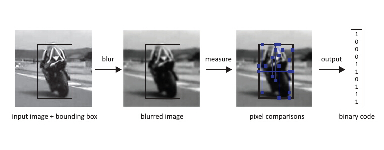
\includegraphics[width=\textwidth]{figs/161002_Thesis_Tracking_Section_04.pdf}
	\caption{集成分类器示意图}
	\label{fig:161002_Thesis_Tracking_Section_04}
\end{figure}

Patch Variance: 首先利用积分图求出当前要分类扫描窗的灰度值期望,再根据期望计算出方差,与原bounding-box的方差作对比,方差小于bounding-box方差的$50\%$的扫描窗都不会通过这个分类器。(这里的阈值是可以调整的)

集成分类器(Ensemble Classifier) 主要采用随机森林(Random Forest )的方法,其中特征选择2bitBP和Pixel Comparisions特征。Pixel Comparisons 的实现方法如下:首先,图像与高斯核进行方差为3像素的卷积,以提高转换稳健性和图像噪声。然后,根据决策树方法进行比较。


Random Forest 方法 :andom Forests方法主要源于BinaryDecision Trees。传统的决策树主要由一系列子二叉树组成,在每一个节点通过简单的YES/NO问题进行分类。在叶子节点,表明数据所属的类型。因此,对于一个决策树而言,一组特征数据通过不同节点的判断,最终得到一个分类结果。通过训练,我们可以根据训练数据的特征,构建一棵“完美”的决策树用于实际应用。但一般而言,单棵决策树训练速度较快,可以快速处理大量数据,但存在过拟合现象,在实际应用中误差较大。为解决单棵决策树存在的缺陷,1995年Ho以及2001年Breiman分别提出采用多个决策树并引入随机特征方法,即Random Forests。其中,通过构建相互独立的多个决策树,从而提高数据处理的多样性;通过在学习过程中引入随机性,来增强系统的鲁棒性。最后,根据少数服从多数的投票原则,判定一个数据的类别。

对样本的处理。Bootstrap Sampling 思想。通过有重复的随机抽取样本,重新组成新的样本集。原始数据集的数学表示如下:
$$\mathbf{\{Dat}{{\mathbf{a}}_{\mathbf{1}}}\mathbf{,Dat}{{\mathbf{a}}_{\mathbf{2}}}\mathbf{,Dat}{{\mathbf{a}}_{\mathbf{3}}}\mathbf{,Dat}{{\mathbf{a}}_{\mathbf{4}}}\mathbf{,Dat}{{\mathbf{a}}_{\mathbf{5}}}\mathbf{,Dat}{{\mathbf{a}}_{\mathbf{6}}}\mathbf{,Dat}{{\mathbf{a}}_{\mathbf{7}}}\mathbf{,Dat}{{\mathbf{a}}_{\mathbf{8}}}\mathbf{,Dat}{{\mathbf{a}}_{\mathbf{9}}}\mathbf{,Dat}{{\mathbf{a}}_{\mathbf{10}}}\mathbf{\}}$$

随机抽取之后的数据集如下:
$$\mathbf{\{Dat}{{\mathbf{a}}_{\mathbf{7}}}\mathbf{,Dat}{{\mathbf{a}}_{\mathbf{6}}}\mathbf{,Dat}{{\mathbf{a}}_{\mathbf{3}}}\mathbf{,Dat}{{\mathbf{a}}_{\mathbf{1}}}\mathbf{,Dat}{{\mathbf{a}}_{\mathbf{1}}}\mathbf{,Dat}{{\mathbf{a}}_{\mathbf{8}}}\mathbf{,Dat}{{\mathbf{a}}_{\mathbf{7}}}\mathbf{,Dat}{{\mathbf{a}}_{\mathbf{2}}}\mathbf{,Dat}{{\mathbf{a}}_{\mathbf{9}}}\mathbf{,Dat}{{\mathbf{a}}_{\mathbf{5}}}\mathbf{\}}$$

可以看到,则随机抽取之后的数据样本集中,不仅样本集的顺序发生了改变,个别样本集也出现了重复。

子特征集的提取。系统不再对全部特征进行训练,而是从中随机选出一个子集进行训练,基于这些子集得到不同类型的决策树。


Random Fern 方法:Random Fern 的思想就是用多个特征组合来表达对象。


\begin{figure}[htb]   
	\centering
	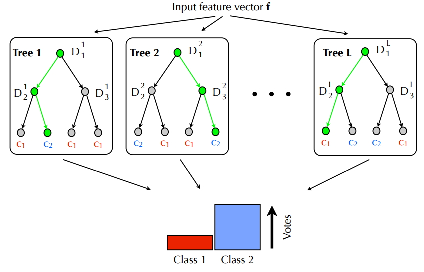
\includegraphics[width=\textwidth]{figs/161002_Thesis_Tracking_Section_05.pdf}
	\caption{集成分类器示意图}
	\label{fig:161002_Thesis_Tracking_Section_05}
\end{figure}

Random Fern 方法基于贝叶斯理论,主要是对简单贝叶斯分类器(Navie Bayes Classifiers)的改进。对于不同的特征$(f_1, f_2, ..., f_N)$而言,分类的最大化这些特征的后验概率:

$$\arg \max_{k}P(C_k|f_1, f_2, ..., f_N)$$

通过贝叶斯公式可以转换为求解最大化极大似然函数与先验概率的乘积

$$\arg \max_{k}P(f_1, f_2, ..., f_N|C_k)P(C_k)$$

这里引入各个特征相互独立的基本假设,方程可以将极大似然函数的求解进一步化简为
$$
P(f_1, f_2, ..., f_N|C_k)=\prod\limits_{i=1}^{N}P(f_i|C_k)
$$
此时,可以得到新的分类公式
$$
\arg\max_kP(C_k)\prod\limits_{i=1}^{N}P(f_i|C_k)
$$
但是在实际问题的求解过程中,每个特征的独立性假设过于严格,因此2007年的CVPR M.Oezuysal中提出Semi-Navie Bayes方法,即将特征进行分组,认为组与组之间保持严格的独立性,而组件的特征相互依赖。假设所有的特征可以分为$L$个组别,每个组别中包含$S$个特征,每个组别被称为Ferns,每一个特征组的表达为
$$
\mathbf{F}_l=\{f_{l,1}, f_{l,2},..., f_{l,S}\}
$$
为了在检测过程中计算便捷,选用二维编码的方式对图像进行描述,因此每一个特征满足$f_n\in\{{0,1}\}$。由此,可以进一步将极大似然函数重新表达
$$
P(f_1, f_2, ..., f_N|C_k)=\prod\limits_{i=1}^{L}P(\mathbf{F}_l|C_k)
$$
基于特征分组的分类公示为
$$
\arg\max_kP(C_k)\prod\limits_{i=1}^{L}P(\mathbf{F}_i|C_k)
$$
在实际训练过程中,由于训练样本数量较少,会导致分类概率为零的情况。因此,我们认为$P(\mathbf{F}|C_k)$符合Dirchlet分布,因此设定一个最小的概率输出
$$
p(\mathbf{F}=z|C_k)=\frac{\mathbb{N}(\mathbf{F}=z|C_k)+1}{\sum_{z=0}^{2^S-1}(\mathbb{N}(\mathbf{F}=z|C_k)+1)}
$$
其中,$\mathbb{N}(\mathbf{F}=z|C_k)$是计算在类别$C_k$情况下,观测到$\mathbf{F}=z$的特征个数。

\subsection{学习器的设计}
学习模块(Leaner)学习过程实时观测追踪器和探测器的执行,并预估探测器的错误,生成训练样例以使能在未来避免类似的错误。学习组件假设追踪器和探测器都有可能出现失败执行,但学习组件的引入可以使得探测器生成更多的追踪目标外观(generalizes to more object appearances),以区别背景。

PN学习即PN learning, P指代Positive Constraint,也称之为P-expert或者growing event,N指代Negative Constraint,也称之为N-expert或者pruning event。

P-expert的作用是发现目标的新的外观(形变),并以此来增加正样本的数量,从而使得检测模块更具鲁棒性;N-expert的作用是生成负的训练样本。N-expert的前提假设是,(被跟踪的)前景目标仅可能出现在视频帧中的一个位置,因此,如果前景目标的位置是确定的,那么其周围必然是负样例。

TLD模块中的PN学习作用是通过对视频序列的在线处理来逐步改善检测模块(TLD中的Detection)的性能。对视频中的每一帧而言,我们希望评估检测模块在当前帧中的误检,并以此来更新目标模型,从而使得在以后的视频帧处理过程中避免类似的错误再次发生。PN学习的关键在于两种类型的“专家(experts)”:P-experts检查那些被检测模块错误分类为正样本(前景目标)的数据;N-experts检查哪些被检测模块错误分类为负样本(背景)的数据;需要提醒的是,无论P-experts还是N-experts都会产生一定的偏差。那么,如果用这些存在偏差的数据来更新检测模块(目标模型),是否会造成检测模型的性能恶化呢?作者经过研究发现,尽管存在误差,在一定条件下,误差是允许的,并且检测模块的性能会因此得到改善。

PN学习包含四个部分:(1)一个待学习的分类器;(2)训练样本集–一些已知类别标签的样本;(3)监督学习–一种从训练样本集中训练分类器的方法;(4)P-N experts–在学习过程中用于产生正(训练)样本和负(训练)样本的表达函数;这四个部分之间的关系如下图所示:

首先根据一些已有类别标记的样本,借助监督学习方法来训练,从而得到一个初始分类器。之后,通过迭代学习,利用上一次迭代得到的分类器对所有的未赋予标签的样本数据进行分类,而P-N experts则找出那些错误分类的样本,并依此来对训练样本集做出修正,使得下一次迭代训练之后得到的分类器的性能有所改善。P-experts将那些被分类器标记为负样本,但根据结构性约束条件应该为正样本的那些样本赋予“正”的标签,并添加到训练样本集中;而N-experts则将那些被分类器标记为正样本,但根据结构性约束条件应该为负样本的那些样本赋予“负”的标签,并添加到训练样本集当中;这也就意味着,P-experts增加了分类器的鲁棒性,而N-experts则增加了分类器的判别能力。

每一个扫描窗口就表示一个图像片(image patch),图像片的类别标签用(b)(c)中的彩色圆点来表示。检测模块对每个图像片的类别赋值过程是彼此独立的,因此,N个扫描窗口就存在个类别标签的组合。而(b)则显示了其中一种可能的类别标签形式,这种类别标签标明,待检测目标在一个视频帧中可能同时出现在好几个区域,并且,待检测目标在相邻视频帧之间的运动没有连续性(例如(b)中最前面的图像中右上角的红色圆点在后面的两个图像中均没有出现),显然,这种类别标签形式是错误的。相反,(c)所示的类别标签形式则显示,每个视频帧中,目标只可能出现在一个区域,并且,相邻视频帧之间检测到的目标区域是连续了,构成了一个目标的运动轨迹。这种性质,我们称之为“结构性”的。PN学习的关键就是找到这种结构性的数据,从而来判别检测模块所产生的错误标签。

刚才的例子表明:P-experts寻找视频序列中的时域上的结构性特征,并且假设目标是沿着轨迹线移动的,即,相邻帧之间的移动很小,且存在一定的相关性。P-experts记录目标在上一帧中的位置,并根据帧与帧之间的跟踪算法(这里采用的是LK光流法)来预测目标在当前帧中的位置。如果检测模块将跟踪算法预测到的目标在当前帧中的位置标记为负标签,那么P-experts就产生一个正的训练样本;N-experts寻找视频序列中的空间域上的结构性特征,并且假设目标在一个视频帧中只可能出现在一个位置。N-experts对检测模块在当前帧中的所有输出结果以及跟踪模块的输出结果进行分析,并找到具有最大可能性的那个区域。当前帧中所有目标可能出现的区域当中,如果某个区域同最大可能性区域之间没有重叠,就将其认定为负样本。另外,具有最大可能性的那个区域,被用于重新初始化跟踪模块。

\section{基于ImageNet神经网络设计方法}

\subsection{搜索区域迭代方法}
搜索区域

红色矩形框:系统识别到的目标。
绿色矩形框:真实参考值。
目的:希望通过对红色矩形的微调,即Bounding Box Regression,更接近绿色矩形。
矩形框的表达一般用四维变量$(x, y, w, h)$表示,即矩形框中心的像素位置以及矩形框的宽度和高度。

迭代方法
- - 寻找一种映射 $f$,使得$f(x_P, y_P, w_P, h_p) = (x_{\hat{G}}, y_{\hat{G}}, w_{\hat{G}}, h_{\hat{G}})$,其中$(x_{\hat{G}}, y_{\hat{G}}, w_{\hat{G}}, h_{\hat{G}}) \approx (x_G, y_G, w_G, h_G)$

- 定义目标区域(Proposal Region) $P=(x_P, y_P, w_P, h_p)$, 真实值区域(Ground-truth Region) $G = (x_G, y_G, w_G, h_G)$,预测区域 $\hat{G}=(x_{\hat{G}}, y_{\hat{G}}, w_{\hat{G}}, h_{\hat{G}})$

- 先平移$(\Delta_x, \Delta_y)$
$$x_{\hat{G}} = w_{P}d_x(P)+x_P$$
$$y_{\hat{G}} = h_{P}d_y(P)+y_P$$

- 再尺度变化$(S_w, S_h)$
$$w_{\hat{G}}=w_{P}exp(d_w(P))$$
$$h_{\hat{G}}=h_{P}exp(d_h(P)$$

- Regression过程

- 输入:$P=(x_P, y_P, w_P, h_p)$这个区域的CNN图像特征,而不是简单的四个点,训练阶段还包括真实值 $T=(x_T, y_T, w_T, h_T)$

- 输出:四个尺度变换$d(P)=(d_x(P), d_y(P), d_w(P), d_h(P))$

$$d_x(P)=(x_{\hat{G}}-x_P)/w_P$$
$$d_y(P)=(y_{\hat{G}}-y_P)/h_P$$
$$d_w(P)=log(w_{\hat{G}}/w_P)$$
$$d_h(P)=log(h_{\hat{G}}/h_P)$$

- 四个基本信息的线性组合方程 $\Phi(P)$

- 在$P$情况下的预测值 $d(P)=\omega^T\Phi(P)$

- 损失函数(可以有很多种)
$$Loss=\sum^N_i(T^{(i)}-\omega^T\Phi(P^{(i)}))^2$$
$$L_{loc}(P,T) = \sum_{i}^N\text{smooth}_{L_1}(T^{(i)}-P^{(i)})$$
$$\text{smooth}_{L_1}(x) = \left \{ \begin{aligned} &0.5x^2 & |x| \le 1\\ &|x|-0.5 & \text{otherwise}\end{aligned} \right.$$
​

- 目标函数
$$\omega^*=\mathop{\arg\min}_{w}\sum^N_i(T^{(i)}-\omega^T\Phi(P^{(i)}))^2+\lambda||\omega||^2$$



\section{基于Siamese神经网络设计方法}

\section{针对图像尺度变换的设计}
在近距离目标跟踪过程中,目标主要发生尺度方面的变化。卷积运算具有平移不变的特性,即



\section{}